\documentclass{report}

\usepackage[a4paper,dvips]{geometry}
\usepackage[utf8]{inputenc}
\usepackage[english]{babel}
\usepackage{graphicx}
\usepackage{multicol}
\usepackage{floatflt}
\usepackage{color}
\usepackage{hyperref}
\usepackage{url}
\usepackage{fancyhdr}
\usepackage{caption}
\usepackage{ucs}
\usepackage{verbatim}
\usepackage{amsmath}
\usepackage{amsfonts}
\usepackage{amssymb}
\usepackage{array}
\usepackage{color}
\usepackage{listings}
\definecolor{colKeys}{rgb}{0,0,1}
\definecolor{colIdentifier}{rgb}{0,0,0}
\definecolor{colComments}{rgb}{0,0.5,1}
\definecolor{colString}{rgb}{0.6,0.1,0.1}
\pagestyle{fancy}
\renewcommand{\headrulewidth}{0pt}
\fancyhead{}
\makeindex
\fancyfoot{}





\begin{document}



%%%%%%%%%%%%%%%%%%%%
% MAIN PAGE %
%%%%%%%%%%%%%%%%%%%%
\begin{titlepage}


\begin{flushleft}
\includegraphics*[width=4cm]{images/logo.jpg} \\
\textsl{12, rue de la Houssinière}\\
\textit{44322 Nantes}
\hrulefill
\end{flushleft}


\vspace{2cm}


\begin{flushleft}

{\fontfamily{ppl}\fontseries{b}\fontsize{1.4cm}{1.65cm}\selectfont AtariGO } \\

\vspace{1cm}

{\Huge Technical Documentation}\\

\vspace{3cm}
{\Large Ngassa Hubert Landry}\\
{\Large Nya Ngaha Chimène-Gaby}\\
{\Large Zerbita Mohamed El Hadi} \\



\end{flushleft}

\vspace{2cm}

\begin{flushleft}
\textsc{Master 1 - ALMA}\\
\hrulefill
\end{flushleft}
\textit{2009-2010}

\end{titlepage}


%%%%%%%%%%%%%%%%%%%%
% CONTENTS %
%%%%%%%%%%%%%%%%%%%%

\tableofcontents
\newpage

%%%%%%%%%%%%%%%%%%%%
% REPORT %
%%%%%%%%%%%%%%%%%%%%
\chapter {Artificial Intelligence}
\addcontentsline{toc}{section}{Artificial Intelligence}

\section* {The specifity of the game}
\addcontentsline{toc}{section}{The specifity of the game}

As an algorithmic game, it is important for us to set a min-max. The
main drawback of the latter with the game of go is the size of the tree. Indeed,
Go game on a 9 * 9 there are 81 possibilities for the games first try. And these
decrease gradually as we advance in the game\\
The tests allow us on a grid of not achieving a vacuum
depth of 3 due to saturation of memory. Suddenly, it becomes almost
obsolete try the min-max depth of 3 from the fact that whatever the
evaluation function will reverse similar notes for several states games
different, and therefore would be less important for informing us very little about
future performance of any tee shot.
Based on these findings it becomes necessary to implement a logic games
allow the most control over the game for a certain number of blows (although
known) to reduce the amount of information to store and begin the evaluation of
game situation by the algorithm of max-min with data (non-strokes and played)
allowing an acceptable cost in time and space.Therefore,we have to offer here
a rather advanced game strategy to best manage the first part of
"Party" Go and min max implemented.\\


\section{Heuristic}
\addcontentsline{toc}{section}{Heuristic}


The heuristic is used to describe the process by which the computer can solve the complex problem of evaluating a state of game.
Its purpose is to calculate a value for a given game state. The more the game state tends towards a conclusive situation for the current player, the more the value must be high.\\

A situation will be conclusive when the current player takes the advantage over his opponent.
Overall a situation is considered conclusive if the player takes more stones than it loses.\\

The heuristic is applied after the first two moves made by the computer, which are determined randomly.\\
\newpage

\section {Main idea for the strategy}
\addcontentsline{toc}{section}{Main idea for the strategy}

The main idea of the strategy used comes from  the following general observation:
For a given state of the goban, the one (the opponent or the machine) which has a group of
freedom pawns is minimal short-handed across the board on the goban. Therefore,it will be
enough for the machine to distinguish two situations when a sudden want to ask about
Goban:\\
\begin{enumerate}
\item If it is short-handed attempt to increase its freedoms.
\item Otherwise it will try to take the most disadvantaged group of the opponent.
\end{enumerate}
Of course, it should avoid the pitfalls causing its release into trouble in the case
where the machine will try to capture a group of pawn adversary\\

To implement this strategy it is our responsibility to know at any moment, the pawns
adverse already played, and those of the machine. To determine the best shot at
play. It will play the shot, according as the game situation needs to expand freedoms
minimum group of the machine or to limit those of the opponent, but with a
priority to the machine. This priority is relatively easy to handle algorithmically, since just start by determining the set of pawns
duty may extend through the machine and not only do if the opponent
is even less favored.
The game is alternatively computer opponent. The opponent starts (he plays
black).\\

This strategy is not very far from the function that we implement by devaluation
thereafter to decide a particular blow to play on the grid. The only difference is that
it is static and does not anticipate unlike min-max, which is essentially a
permanent anticipation. This strategy is therefore static can not guarantee for
when a success every time but plays a logic very consistent.
If the player fails to catch shots after x game, the min-max take care of
Following the game are presented in what follows the implementation of the game from this
time. This is essentially the min-max and the evaluation function.\\



\chapter{Implementation}
\addcontentsline{toc}{chapter}{Implementation}

\section*{Program Architecture}
\addcontentsline{toc}{section}{Program Architecture}

\section{Packages}
\addcontentsline{toc}{section}{Packages Architecture}

Our program is organized in six packages,which are be described as following:\\
\begin{itemize}
\item {\fontseries{b} {\large fr.alma.ia}:  which is responsible for calculations of artificial intelligence.
This package contains classes for managing artificial intelligence, are the strategy and
management and detection of pieces or groups of pieces and the MinMax and function
Assessment:
\begin {itemize}
   \item Ia: The class of the evaluation function.
   \item MinMax: The class of the MinMax algorithm.
   \item OutilsIA: class that contains some useful methods.
\end{itemize} 
}
\item {\fontseries{b} {\large fr.alma.ihm}:  representing the user interface which communicate with the game}\\
\item {\fontseries{b} {\large fr.alma.images}:  which represents the different images used for the user interface}\\
\item {\fontseries{b} {\large fr.alma.jeu}:  which represents the rules and mechanisms of the game atarigo.
  This package contains classes that manage the game, which are:
\begin {itemize}
   \item Pion: class that handles the pawn.Caracterised by its color and its position on the goban.
   \item Grille: class that allows the specification of the grid.
   \item Game: class that handles the different rules of the game, it detects
       Catch and suicides.
   \item LibertePion: manages the freedoms pawns.
   \item OutilsJEU: contains some useful methods to manage the game
  \item Tour: Enumeration to represent the tour players.
   \item Couleur Enumeration for the color of the pieces.
\end{itemize} 
}

\item {\fontseries{b} {\large fr.alma.main}:  This package contains the main class where there is the main method that allows to launch the application.}\\
\item {\fontseries{b} {\large fr.alma.stucture}:  which represents the structure of the tree buit during the game between a human being and a computer.
This package contains classes that allow the construction of the tree and
MinMax algorithm for current classes are:
\begin {itemize}
     \item Noeud: class accounted for a node in the tree.
     \item Arbre: This class is used to build a tree from a state of the grid,
         can also applied a MinMax tree
\end{itemize} 
}
\end{itemize}


\section{Class Diagrams}
\addcontentsline{toc}{section}{Class Diagrams}


\subsection*{iaClassDiagram}
\addcontentsline{toc}{subsection}{iaClassDiagram}
\begin{center}
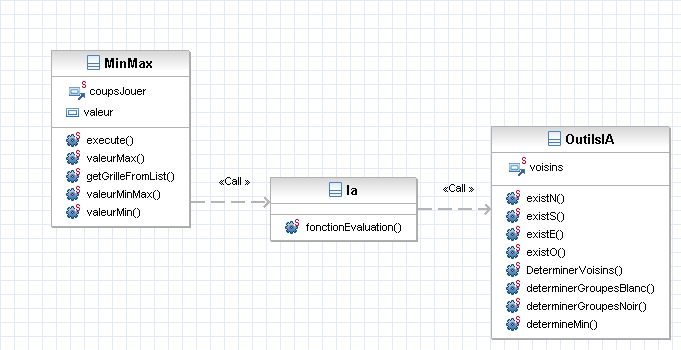
\includegraphics[scale=0.70]{images/fralmaiaClassDiagram}
\captionof{figure}{Class diagram of IA}
\end{center}


\subsection*{ihmClassDiagram}
\addcontentsline{toc}{subsection}{ihmClassDiagram}
\begin{center}
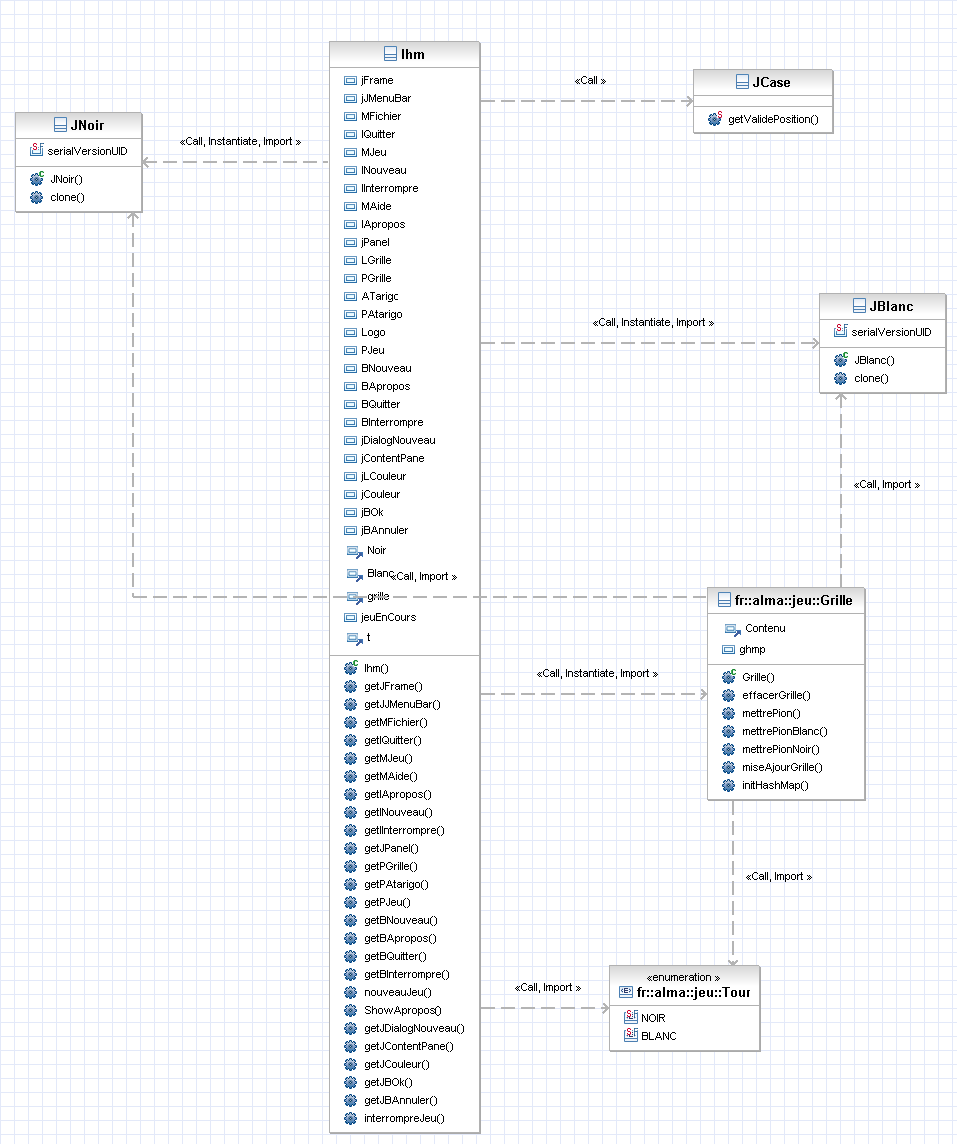
\includegraphics[scale=0.30]{images/fralmaihmClassDiagram}
\captionof{figure}{Class diagram of Ihm}
\end{center}



\subsection*{jeuClassDiagram}
\addcontentsline{toc}{subsection}{jeuClassDiagram}
\begin{center}
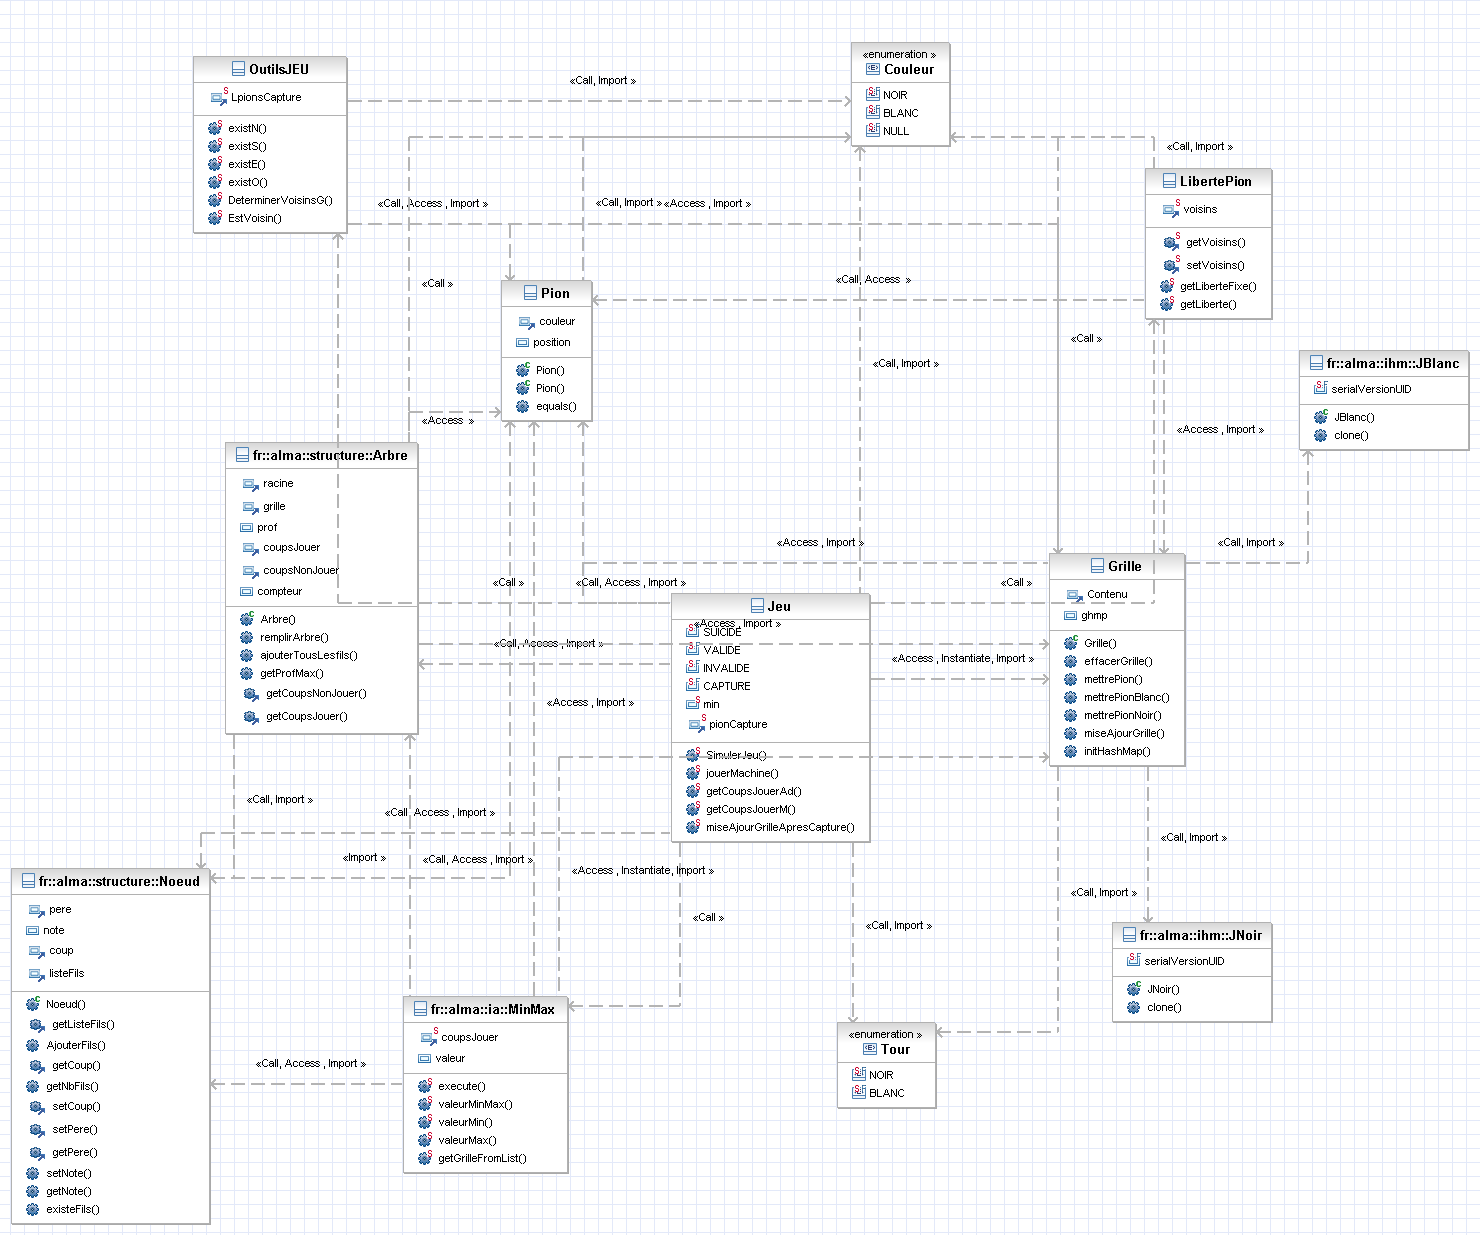
\includegraphics[scale=0.50]{images/fralmajeuClassDiagram}
\captionof{figure}{Class diagram of Jeu}
\end{center}



\subsection*{mainClassDiagram}
\addcontentsline{toc}{subsection}{mainClassDiagram}
\begin{center}
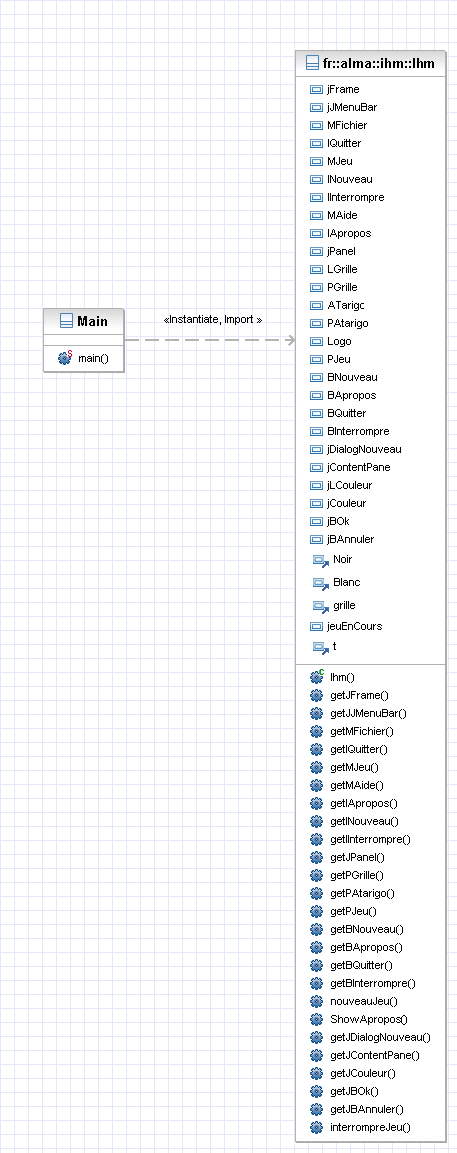
\includegraphics[scale=0.50]{images/fralmamainClassDiagram}
\captionof{figure}{Class diagram of Main}
\end{center}



\subsection*{structureClassDiagram}
\addcontentsline{toc}{subsection}{structureClassDiagram}
\begin{center}
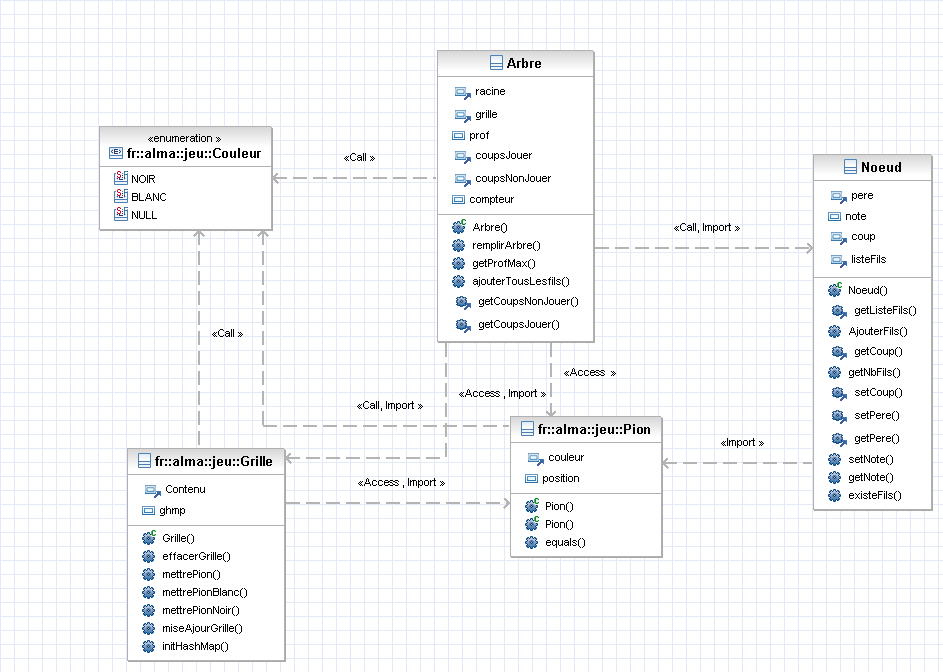
\includegraphics[scale=0.50]{images/fralmastructureClassDiagram}
\captionof{figure}{Class diagram of Structure}
\end{center}







\chapter{Algorithms}
\addcontentsline{toc}{chapter}{Algorithms}

\section{MinMax Algorithm }
\addcontentsline{toc}{section}{MinMax Algorithm }

It's a recursive algorithm for choosing the next move in an n-player game, usually a two-player game. A value is associated with each position or state of the game. This value is computed by means of a position evaluation function and it indicates how good it would be for a player to reach that position. The player then makes the move that maximizes the minimum value of the position resulting from the opponent's possible following moves.\\

\begin{center}
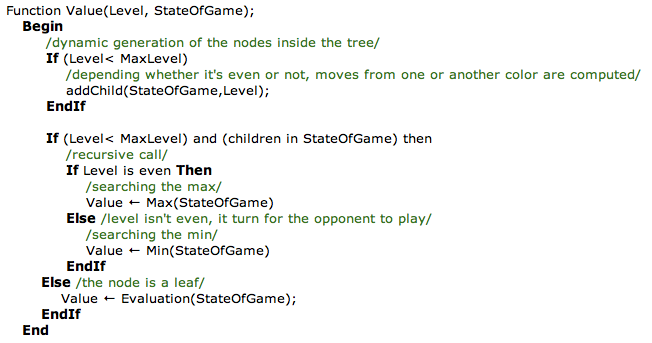
\includegraphics[scale=0.60]{images/MinMax.png}
\captionof{figure}{MinMax Algorithm}
\end{center}

\vspace{1cm}

We present in this part the implementation of the min-max that we have produced.
Indeed, for the sake of saving space we use the tree must have a
structure as light as possible (store the minimum information in a node) to
use on a fairly large number of shots.
To construct the tree of min-max, we use a trick that allows us to do
reconstruct the grid once in the leaves. Indeed for a current game state, we
gets all the play opportunities still available on the Goban. And then we
construct a tree where each node is one of the shots still stored on the Goban.
This allows us to store more information than if it were a store
Goban by an entire node.
Starting from the root to a leaf node all through, added to the Goban
gives the initial position reached in the Goban games that can be evaluated.\\

For a grid when you're in a leaf,it will suffice to
alternatively put pawns in the grid. So in a leaf, we construct a grid
supplementing that they had initially. The grid obtained(i.e the state of the goban at a given time of the game) in a leaf is evaluated and
whichever is stored in it (the leaf). It uses the algorithm of min-max to rise
up the appropriate value to determine the ideal shot to play.\\

\section*{Evaluation Fonction }
It is based on the same principle that the strategy used previously. Indeed it
takes into account three important aspects of the game of go:\\

\begin{itemize}
   \item Knowledge Representation.
    \item Concepts of groups.
    \item From chains stones.
\end{itemize}

She tries to give each group of stones assessed in terms of life or death
(Concept of freedom of a group).
The implementation, rather powerful and simple is the following:\\

\begin{itemize}
    \item From a complete grid, determine the groups of pieces (and those opposing
        the machine).
    \item Determine the group of pieces that the minimum freedom in the adversary (Mina).
   \item Identify the group that has minimal freedom for the machine (Minmi).
    \item Return  {\fontseries{b} "Minmi - Mina"} or {\fontseries{b} "Minmi K *-K '* Mina"}
\end{itemize}

Where k and k 'are the relative importance to strokes to reach the current
grid. We just use the first.\\
Notes:
\begin{itemize}
    \item It returns a value that truly represents the maximum degree of relevance
        a position of the grid.
    \item With a value of 0 it allows the machine to hold the game 
\end{itemize}


\section{AlphaBeta Algorithm  }
\addcontentsline{toc}{section}{AlphaBeta Algorithm  }

Alpha-beta pruning is a search algorithm which seeks to reduce the number of nodes that are evaluated in the search tree by the minimax algorithm.

\begin{center}
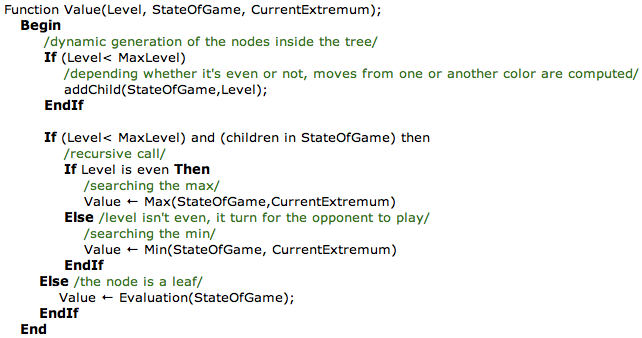
\includegraphics[scale=0.60]{images/AlphaBeta.png}
\captionof{figure}{AlphaBeta Algorithm}
\end{center}


\chapter {Perspectives}
\addcontentsline{toc}{chapter}{Perspectives}


For an artificial intelligence playing a game, time is critical. With infinite time, it is shown that the MinMax method (based on a good heuristic) will always find the ideal configuration of play. But the time allowed for reflection during a game is rarely infinite. Therefore, the more the computer can process data faster, the more it will deepen its reflection (and be stronger). \\

For this, two parameters are taken into account: The computational complexity mentioned above, but also the complexity in memory.
From the perspective of memory, the main issue is the storage representation of a Goban. Several solutions are available to us: \\

\begin{enumerate}
\item Use a square matrix modeling entire goban (a grid of color and empty squares).
\item Use a list of played stones only (couples position / color).
\end{enumerate}
Both solutions have each an argument in their favor and one against them. 
Indeed, the matrix provides a constant time access, access is O(1). For cons, the Goban still occupies the same memory space whether it's empty or full and demands a contiguous memory space . It is therefore an important loss. \\



\end{document}

